\documentclass[12pt,a4paper]{article}

\usepackage[utf8]{inputenc}
\usepackage[T1]{fontenc}
\usepackage[italian]{babel}
\usepackage{geometry}
\usepackage{setspace}
\usepackage{graphicx}
\usepackage{titlesec}
\usepackage{tocloft}
\usepackage{hyperref}
\usepackage{csquotes}

\geometry{top=2.5cm,bottom=2.5cm,left=2.5cm,right=2.5cm}
\onehalfspacing
\setlength{\parindent}{0.5cm}
\setlength{\parskip}{0pt}

\hypersetup{
  colorlinks=true,
  linkcolor=black,
  urlcolor=blue,
  pdftitle={Relazione di fine tirocinio - Sistema di gestione del processo di presa in carico PDTA},
  pdfauthor={Daniele Lucifora}
}

\titleformat{\section}
  {\normalfont\bfseries\Large}
  {\thesection}{0.5em}{}

\begin{document}

% ---------------- FRONTESPIZIO ----------------
\begin{titlepage}
    \centering

    {\large UNIVERSITA DEGLI STUDI DI CATANIA\par}
    \vspace{0.3cm}
    {\normalsize Dipartimento di Ingegneria Elettrica Elettronica e Informatica\par}
    {\normalsize Corso di Laurea Magistrale in Ingegneria informatica\par}

    \vspace{1.2cm}

    
\includegraphics[width=0.38\textwidth]{assets/unict-logo.png}\par

    \vspace{1.2cm}

    {\Large\bfseries Relazione finale di tirocinio curriculare\par}
    \vspace{0.8cm}

    {\LARGE\bfseries Progettazione e Implementazione di Workflow Sanitari con Camunda BPM\par}

    \vspace{0.6cm}

    {\large Modellazione BPMN 2.0, integrazione software e monitoraggio di processi clinico-organizzativi\par}

    \vfill

    \begin{flushleft}
    \normalsize
    Candidato: Daniele Lucifora\\
    Matricola: 1000066513\\
    Tutor universitario: Prof. Giovanni Morana\\
    Tutor aziendale: Ing. Giovanni Cammarata\\
    Azienda ospitante: Vyxel s.r.l.\\
    Anno Accademico: 2024/2025
    \end{flushleft}

\end{titlepage}

\clearpage
\pagenumbering{arabic}
\setcounter{page}{2}

% ---------------- INDICE ----------------
\tableofcontents

\clearpage

% ---------------- INTRODUZIONE ----------------
\section*{Introduzione}
\addcontentsline{toc}{section}{Introduzione}

Il presente elaborato descrive il percorso di tirocinio curriculare svolto presso Vyxel s.r.l., finalizzato alla tesi, e incentrato sulla progettazione e implementazione del Sistema di gestione del processo di presa in carico PDTA. Il lavoro si inserisce nell'area aziendale dedicata allo sviluppo di soluzioni software e data-driven, con attenzione all'integrazione di componenti avanzati, alla gestione di infrastrutture tecnologiche e alla costruzione di architetture scalabili orientate ai processi.

Per \emph{PDTA} (Percorso Diagnostico Terapeutico Assistenziale) si intende uno strumento organizzativo che definisce in modo strutturato le fasi di presa in carico, diagnosi, trattamento e follow-up del paziente, coordinando ruoli clinici differenti secondo criteri di appropriatezza, qualità e continuità assistenziale.

Il dominio applicativo scelto, quello dei protocolli sanitari PDTA, ha richiesto di conciliare rigore procedurale e flessibilità implementativa. La presenza di ruoli diversi, vincoli decisionali e dipendenze temporali rende infatti questo ambito particolarmente adatto a una sperimentazione concreta delle metodologie BPM e degli strumenti di orchestrazione dei processi.

% ---------------- CAPITOLI ----------------
\section{Contesto aziendale e finalita del tirocinio}

Vyxel s.r.l. opera nello sviluppo di soluzioni software e data-driven con integrazione di componenti intelligenti, gestione di infrastrutture storage e ambienti bare-metal, con particolare attenzione a workflow applicativi e sistemi orientati ai processi. Questo quadro ha orientato il tirocinio verso una visione ingegneristica completa, in cui la qualità del risultato dipende dall'allineamento tra modellazione formale, implementazione applicativa e osservabilità operativa.

La finalità principale del percorso è stata la realizzazione di un workflow sanitario eseguibile e verificabile, capace di rappresentare il processo di accettazione PDTA con valutazione GOM, ruoli distinti e vincoli decisionali espliciti.

\section{Obiettivi formativi e professionali}

Gli obiettivi di base hanno riguardato la comprensione dei principi BPM, l'uso del linguaggio BPMN 2.0 e l'analisi del dominio dei protocolli sanitari. Sul piano tecnico-professionale, il tirocinio ha mirato alla progettazione di workflow complessi in Camunda, all'implementazione di componenti software per prenotazioni e referti, alla verifica funzionale del processo e alla valutazione delle performance. In parallelo, gli obiettivi trasversali hanno incluso pianificazione delle attivita, comunicazione tecnica, gestione delle priorità, collaborazione e autonomia operativa.

L'insieme di questi obiettivi è stato perseguito in modo progressivo, con verifiche periodiche e confronto costante con il tutor aziendale, Ing. Giovanni Cammarata.

\section{Metodologia e approccio di lavoro}

Il lavoro è stato organizzato in iterazioni successive, partendo da uno studio preliminare su Spring Boot e Camunda e passando poi alla traduzione dei requisiti di dominio in modello BPMN eseguibile. Ogni incremento ha previsto una fase di implementazione, una fase di verifica funzionale e una fase di consolidamento, con particolare attenzione alla leggibilita del codice e alla tracciabilità delle decisioni progettuali.

Questo approccio ha permesso di gestire la complessità in modo controllato, riducendo il rischio di disallineamento tra modello di processo e comportamento runtime e favorendo una crescita progressiva della robustezza complessiva del sistema.

\section{Architettura del Sistema di gestione del processo di presa in carico PDTA}

Il progetto è stato sviluppato con Java 21 e Spring Boot, utilizzando Camunda Platform 8 come motore di orchestrazione dei processi. La persistenza è stata realizzata con H2 file-based in ambiente prototipale, scelta adeguata alla rapidità di iterazione e alla semplicità di setup. Maven ha supportato la gestione delle dipendenze e del ciclo di build.

La struttura applicativa è stata mantenuta modulare, separando le componenti di dominio, i servizi applicativi, i worker e le interfacce operative. Questa organizzazione ha favorito manutenibilità, testabilità e chiarezza nell'evoluzione del codice.

\section{Modellazione BPMN 2.0 del workflow sanitario}

La modellazione BPMN ha formalizzato il percorso di presa in carico PDTA, includendo triage iniziale, verifica criteri di inclusione, validazioni specialistiche e gestione degli esami diagnostici. L'uso di gateway decisionali e task di ruolo ha consentito di rappresentare in modo esplicito i vincoli procedurali, riducendo ambiguità interpretative.

Durante il consolidamento è emersa la necessità di separare con maggiore rigore la fase di scheduling diagnostico dalla fase di refertazione, poichè le due attività non coincidono temporalmente. Questa riflessione metodologica ha costituito un passaggio importante, evidenziando il valore del BPMN non solo come strumento descrittivo ma come modello eseguibile aderente al comportamento atteso nel dominio reale.

\begin{figure}[h]
  \centering
  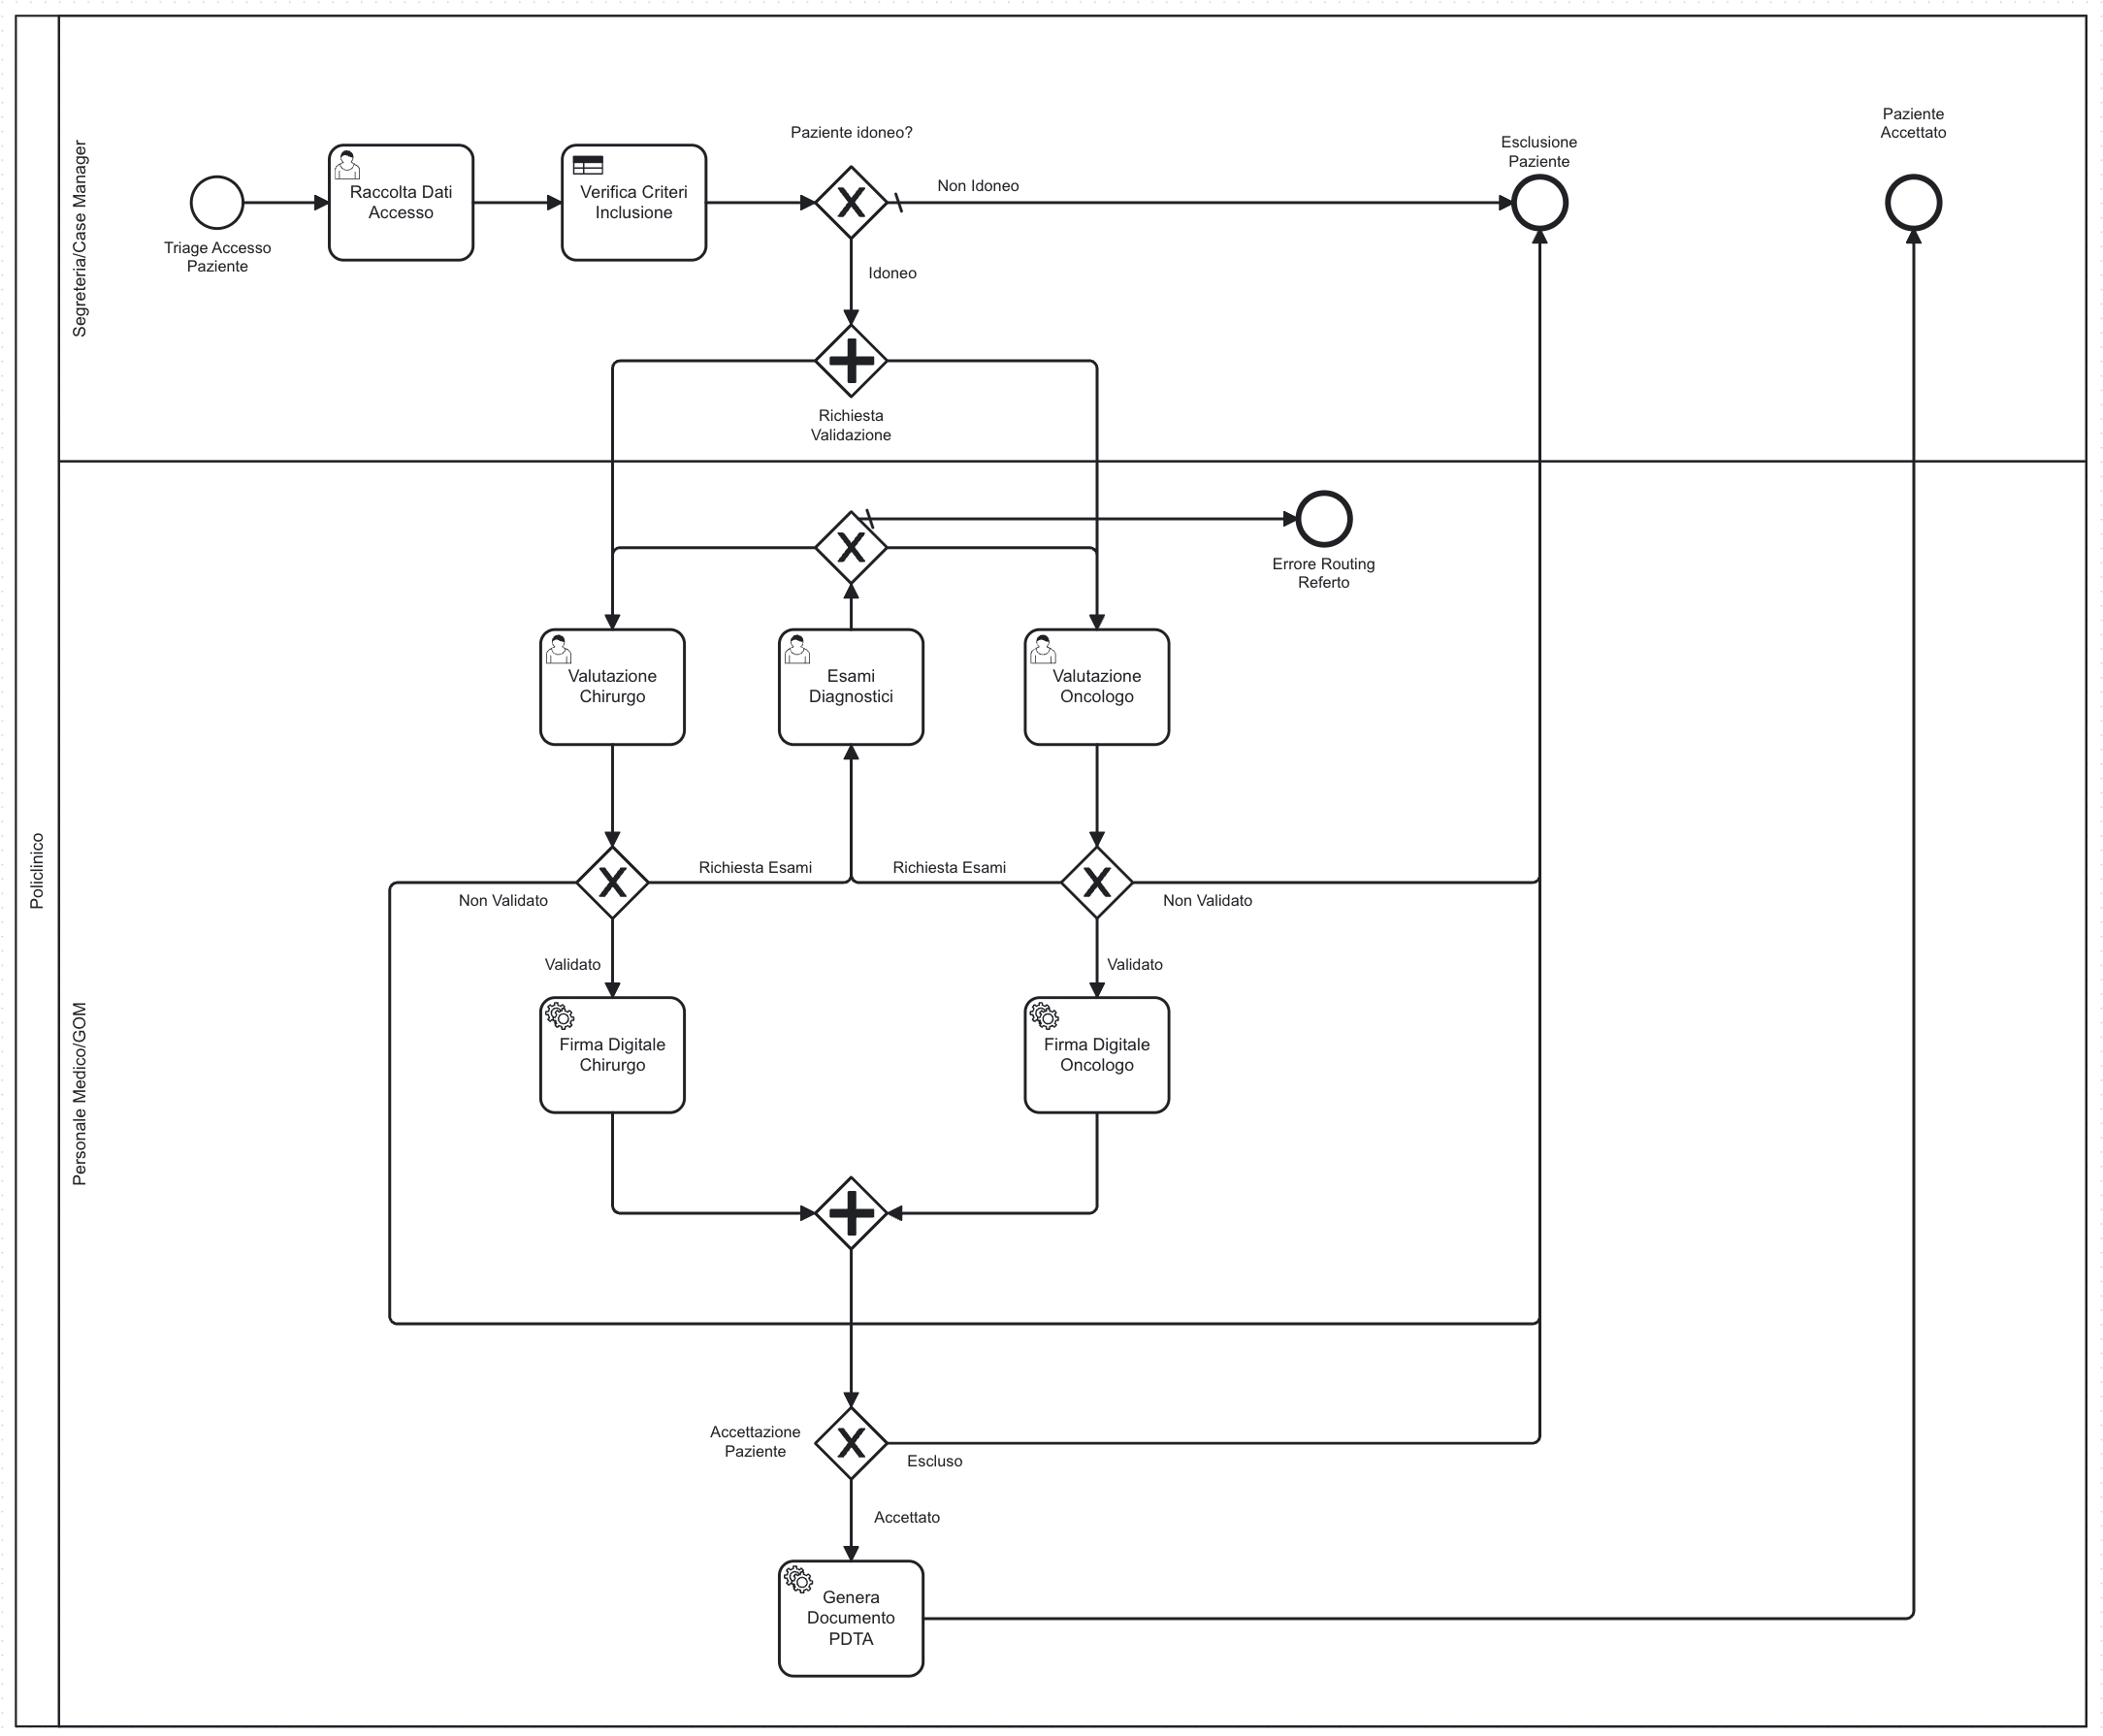
\includegraphics[width=0.95\textwidth]{presa_in_carico_pdta.png}
  \caption{Workflow BPMN del processo \emph{presa\_in\_carico\_pdta}: dal triage iniziale alla decisione finale di accettazione o esclusione del paziente.}
  \label{fig:workflow-bpmn-pdta}
\end{figure}

La figura mostra la logica complessiva del flusso: avvio con raccolta dati e verifica DMN di eleggibilità, valutazione parallela di chirurgo e oncologo, eventuale ciclo degli esami diagnostici con rientro verso lo specialista richiedente, convergenza sulle firme digitali e generazione del documento PDTA nei casi approvati.

\section{Implementazione software e integrazione applicativa}

L'implementazione ha riguardato la costruzione delle entità principali del sistema e dei relativi servizi: risorse diagnostiche, protocolli d'esame, slot di prenotazione, eventi di audit e snapshot KPI. Le operazioni applicative sono state integrate nel workflow in modo da rispettare responsabilità e vincoli dei diversi ruoli coinvolti.

Le interazioni operative sono state supportate da componenti CLI dedicate, utili per simulare i flussi reali e validare l'end-to-end del processo. In questa fase si è lavorato anche sul miglioramento progressivo della struttura del codice, con refactoring mirati alla chiarezza e alla riduzione di accoppiamenti non necessari.

\section{Testing, verifica funzionale e qualità}

La verifica è stata condotta attraverso test funzionali sui casi principali e sui percorsi decisionali piu sensibili. L'attenzione si è concentrata sulla coerenza delle variabili di processo, sulla correttezza delle transizioni tra stati e sull'allineamento tra comportamento atteso e comportamento osservato in esecuzione.

Il percorso ha evidenziato come, nei sistemi process-driven, la qualità dipenda in modo determinante dalla coerenza tra modello BPMN e logica applicativa. Per questo motivo il testing è stato trattato come attività continua, non solo finale, a supporto diretto delle decisioni progettuali.

\section{Monitoraggio, KPI e valutazione delle performance}

Per rendere il sistema valutabile nel tempo è stata introdotta una componente di KPI giornalieri aggregati. Questa scelta ha migliorato la leggibilità dei trend operativi e ha ridotto il costo delle interrogazioni su eventi storici, offrendo una base solida per reporting e analisi.

E' stata inoltre considerata l'integrazione di strumenti di monitoraggio time-series, in particolare Prometheus, in logica affiancata al database applicativo. La valutazione tecnica ha confermato che la persistenza relazionale resta appropriata per i dati di dominio, mentre il monitoraggio real-time rappresenta un'estensione utile per metriche operative, alerting e osservabilità avanzata.

\section{Competenze acquisite e risultati raggiunti}

Il tirocinio ha consentito di consolidare competenze concrete nella modellazione BPMN 2.0, nell'uso di Camunda per design e orchestrazione, nella progettazione software orientata al dominio e nello sviluppo di codice manutenibile e testabile. Sono state inoltre rafforzate pratiche professionali legate a versionamento, documentazione tecnica e comunicazione dello stato di avanzamento.

Sul piano organizzativo, il percorso ha favorito una crescita nell'autonomia operativa, nella pianificazione del lavoro e nella gestione delle priorità, con beneficio diretto sulla qualità delle decisioni e sulla continuità delle attività.

\section{Criticità affrontate e soluzioni adottate}

Le principali criticità hanno riguardato l'allineamento tra complessità del dominio sanitario e semplicità prototipale, oltre alla gestione delle dipendenze temporali nel flusso diagnostico. Questi aspetti sono stati affrontati con una strategia di miglioramento incrementale, basata su refactoring mirati, verifiche frequenti e aggiornamento continuo della documentazione tecnica.

Il confronto periodico con il tutor aziendale ha avuto un ruolo decisivo nel mantenere coerenza metodologica e orientamento ai risultati, trasformando le criticità in occasioni di consolidamento delle competenze.

\section*{Conclusioni}
\addcontentsline{toc}{section}{Conclusioni}

Il tirocinio svolto presso Vyxel s.r.l. ha raggiunto in modo sostanziale gli obiettivi formativi, tecnico-professionali e trasversali prefissati. Il Sistema di gestione del processo di presa in carico PDTA ha dimostrato l’efficacia di un approccio process-driven nella gestione di workflow sanitari, offrendo una base concreta per ulteriori sviluppi sia accademici sia applicativi. L’esperienza ha permesso di acquisire competenze avanzate nella modellazione dei processi, nello sviluppo software e nella gestione delle problematiche tipiche dei sistemi complessi.

In prospettiva, gli sviluppi più rilevanti riguardano il rafforzamento della separazione temporale delle fasi diagnostiche nel modello BPMN, l’estensione della copertura di test automatici, l’incremento dell’osservabilità real-time e la progressiva evoluzione verso interfacce GUI role-based. Tali direzioni risultano coerenti con il percorso svolto e con gli standard attesi in contesti professionali complessi. Il tirocinio ha rappresentato un’importante occasione di crescita personale e professionale, fornendo una solida base per affrontare con successo le sfide future nel campo dell’ingegneria del software e della gestione dei processi.

\end{document}
